\documentclass[12pt]{article}

%environnement
\usepackage[letterpaper,margin=1in]{geometry}
\usepackage[utf8]{inputenc}
\usepackage{fontspec}
\usepackage[english]{babel}
\usepackage[parfill]{parskip}
\usepackage[style=ieee,backend=bibtex]{biblatex} %gestion bib
\usepackage{listings}
\usepackage{hyperref}
\usepackage[toc,acronym]{glossaries}
\usepackage[framemethod=TikZ]{mdframed} 
\usepackage{todonotes}
\usepackage[section]{placeins}
\hypersetup{
  pdftitle={},
  pdfborder={0 0 0}, %epaisseur box
  pdfauthor={Thomas LUINAUD},
}
\usepackage{tikz,tkz-tab}%package pour les tableaux de variations et de signes%
\usetikzlibrary{babel}
\usepackage{modules/tikzNetwork}
\usepackage{circuitikz}
\usetikzlibrary{positioning, automata, graphs, trees, fit, arrows.meta, shapes}
\usetikzlibrary{backgrounds,patterns,matrix,calc,shadows,plotmarks, circuits.logic.US}
\usetikzlibrary{decorations}
\usepackage{multirow}
\usepackage{modules/moeptikz}
%\usepackage{tabularx}
 %this file contains shape declaration and macro that define 
 %basic computer science shape for Hardware design.
 %this file should be include in the preamble
 
 \catcode`@=11

\pgfkeys{%
  /pgf/logicalbloc io north/.initial=5,
%  /pgf/logicalbloc io south/.initial=10,
%  /pgf/logicalbloc io east/.initial=10,
  /pgf/logicalbloc io west/.initial=10,
  /pgf/logicalbloc io north spacing/.initial=0.15cm,
%  /pgf/logicalbloc io south spacing/.initial=0.25cm,
%  /pgf/logicalbloc io east spacing/.initial=0.25cm,
  /pgf/logicalbloc io west spacing/.initial=0.20cm
}
\def\maxpins{100}


%stdChip
\pgfdeclareshape{logicalbloc}{
	\savedanchor\centerpoint{% 
		\pgf@x=.5\wd\pgfnodeparttextbox%
		\pgf@y=.5\ht\pgfnodeparttextbox%
		\advance\pgf@y by-.5\dp\pgfnodeparttextbox%
	  }
	  \anchor{center}{\centerpoint}
	  
	  \saveddimen\height{%
		\pgfmathsetlength\pgf@x{(\pgfkeysvalueof{/pgf/logicalbloc io west}+1)*\pgfkeysvalueof{/pgf/logicalbloc io west spacing}}%
	  }
	  \saveddimen\width{%
		\pgfmathsetlength\pgf@y{(\pgfkeysvalueof{/pgf/logicalbloc io north}+1)*\pgfkeysvalueof{/pgf/logicalbloc io north spacing}}%
	  }
	  \saveddimen{\yspacing}{\pgfmathsetlength\pgf@x{\pgfkeysvalueof{/pgf/logicalbloc io west spacing}}}	  
	  \saveddimen{\xspacing}{\pgfmathsetlength\pgf@y{\pgfkeysvalueof{/pgf/logicalbloc io north  spacing}}}
	  
	  \backgroundpath{%
		\pgfpathrectanglecorners{\pgfpointadd{\centerpoint}{\genbottomleftpoint}}%
		{\pgfpointadd{\centerpoint}{\gentoprightpoint}}%
	  }
 

	  \pgfmathloop%
	  \ifnum\pgfmathcounter>\maxpins\relax% 
	  \else%
		% Need to expand \pgfmathcounter
		\edef\marshal{\noexpand\anchor{io east \pgfmathcounter}}%
		\expandafter\marshal\expandafter{\expandafter\chippinanchorright\expandafter{\pgfmathcounter}}%
	  \repeatpgfmathloop%
	  
	  \pgfmathloop%
	  \ifnum\pgfmathcounter>\maxpins\relax% 
	  \else%
		% Need to expand \pgfmathcounter
		\edef\marshal{\noexpand\anchor{io north \pgfmathcounter}}%
		\expandafter\marshal\expandafter{\expandafter\chippinanchorupper\expandafter{\pgfmathcounter}}%
	  \repeatpgfmathloop%
	  
	  \pgfmathloop%
	  \ifnum\pgfmathcounter>\maxpins\relax% 
	  \else%
		% Need to expand \pgfmathcounter
		\edef\marshal{\noexpand\anchor{io south \pgfmathcounter}}%
		\expandafter\marshal\expandafter{\expandafter\chippinanchorbottom\expandafter{\pgfmathcounter}}%
	  \repeatpgfmathloop%
	  
	  \pgfmathloop%
	  \ifnum\pgfmathcounter>\maxpins\relax% 
	  \else%
		% Need to expand \pgfmathcounter
		\edef\marshal{\noexpand\anchor{io west \pgfmathcounter}}%
		\expandafter\marshal\expandafter{\expandafter\chippinanchorleft\expandafter{\pgfmathcounter}}%
	  \repeatpgfmathloop%
}

\def\genbottomleftpoint{%
%	\pgfmathsetlength{pgf@xb}{(\pgfkeysvalueof{/pgf/logicalbloc io north}+1)*\pgfkeysvalueof{/pgf/logicalbloc io north spacing}}%
%	\pgfmathsetlength{pgf@yb}{(\pgfkeysvalueof{/pgf/logicalbloc io west}+1)*\pgfkeysvalueof{/pgf/logicalbloc io west spacing}}%
%	\setlength{\pgf@xa}{1cm}
%	\setlength{\pgf@ya}{1cm}
%	\if \pgf@xb<\pgf@xa
%		\if \pgf@yb<\pgf@ya
%			\pgfpoint{-0.5cm}{-0.5cm}
%		\else
%			\pgfpoint{-0.5cm}{-(\pgfkeysvalueof{/pgf/logicalbloc io west}+1)*\pgfkeysvalueof{/pgf/logicalbloc io west spacing}/2}
%		\fi
%	\else
%		\if \pgf@yb<\pgf@ya
%			\pgfpoint{-(\pgfkeysvalueof{/pgf/logicalbloc io north}+1)*\pgfkeysvalueof{/pgf/logicalbloc io north spacing}/2}{-0.5cm}
%		\else
			\pgfpoint{-((\pgfkeysvalueof{/pgf/logicalbloc io north}+1)*\pgfkeysvalueof{/pgf/logicalbloc io north spacing})/2}{-((\pgfkeysvalueof{/pgf/logicalbloc io west}+1)*\pgfkeysvalueof{/pgf/logicalbloc io west spacing})/2}
%		\fi
%	\fi
}
\def\gentoprightpoint{%
%	\if {\pgfkeysvalueof{/pgf/logicalbloc io west} < \pgfkeysvalueof{/pgf/logicalbloc io east}}
%		\setlength{\pgf@xc}{1cm}
%	\else
%		\setlength{\pgf@xc}{1cm}
%	\fi
%	\if
%		\setlength{\pgf@xc}{1cm}
%	\else
%		\setlength{\pgf@xc}{1cm}
%	\fi
%	\pgfmathsetlength{pgf@xb}{(\pgfkeysvalueof{/pgf/logicalbloc io north}+1)*\pgfkeysvalueof{/pgf/logicalbloc io north spacing}}%
%	\pgfmathsetlength{pgf@yb}{(\pgfkeysvalueof{/pgf/logicalbloc io west}+1)*\pgfkeysvalueof{/pgf/logicalbloc io west spacing}}%
%	\setlength{\pgf@xa}{1cm}
%	\setlength{\pgf@ya}{1cm}
%	\if \pgf@xb<\pgf@xa
%		\if \pgf@yb<\pgf@ya
%			\pgfpoint{0.5cm}{0.5cm}
%		\else
%			\pgfpoint{0.5cm}{(\pgfkeysvalueof{/pgf/logicalbloc io west}+1)*\pgfkeysvalueof{/pgf/logicalbloc io west spacing}/2}
%		\fi
%	\else
%		\if \pgf@yb<\pgf@ya
%			\pgfpoint{(\pgfkeysvalueof{/pgf/logicalbloc io north}+1)*\pgfkeysvalueof{/pgf/logicalbloc io north spacing}/2}{0.5cm}
%		\else
			\pgfpoint{((\pgfkeysvalueof{/pgf/logicalbloc io north}+1)*\pgfkeysvalueof{/pgf/logicalbloc io north spacing})/2}{((\pgfkeysvalueof{/pgf/logicalbloc io west}+1)*\pgfkeysvalueof{/pgf/logicalbloc io west spacing})/2}
%		\fi
%	\fi
}


\def\genpointbottom#1{
\pgfpoint{(\pgfkeysvalueof{/pgf/logicalbloc io north}+1)*\pgfkeysvalueof{/pgf/logicalbloc io north spacing}/2-#1*\xspacing}{-(\pgfkeysvalueof{/pgf/logicalbloc io west}+1)*\pgfkeysvalueof{/pgf/logicalbloc io west spacing}/2}
}

\def\chippinanchorbottom#1{%
	  % When this macro is called,
	  % \centerpoint, \height and \chipspacing will be defined.
	  %\pgfpointadd{\centerpoint}{\pgfpoint{\width/2-#1*\xspacing}{-\height/2}}%
	  \pgfpointadd{\centerpoint}{\genpointbottom{#1}}%
}

\def\genpointupper#1{
\pgfpoint{(\pgfkeysvalueof{/pgf/logicalbloc io north}+1)*\pgfkeysvalueof{/pgf/logicalbloc io north spacing}/2-#1*\xspacing}{(\pgfkeysvalueof{/pgf/logicalbloc io west}+1)*\pgfkeysvalueof{/pgf/logicalbloc io west spacing}/2}
}

\def\chippinanchorupper#1{%
	  % When this macro is called,
	  % \centerpoint, \height and \chipspacing will be defined.
	  \pgfpointadd{\centerpoint}{\genpointupper{#1}}%
}

\def\genpointleft#1{
\pgfpoint{-(\pgfkeysvalueof{/pgf/logicalbloc io north}+1)*\pgfkeysvalueof{/pgf/logicalbloc io north spacing}/2}{(\pgfkeysvalueof{/pgf/logicalbloc io west}+1)*\pgfkeysvalueof{/pgf/logicalbloc io west spacing}/2-#1*\yspacing}
}

\def\chippinanchorleft#1{%
	  % When this macro is called,
	  % \centerpoint, \height and \chipspacing will be defined.
	  \pgfpointadd{\centerpoint}{\genpointleft{#1}}%
}

\def\genpointright#1{
\pgfpoint{(\pgfkeysvalueof{/pgf/logicalbloc io north}+1)*\pgfkeysvalueof{/pgf/logicalbloc io north spacing}/2}{(\pgfkeysvalueof{/pgf/logicalbloc io west}+1)*\pgfkeysvalueof{/pgf/logicalbloc io west spacing}/2-#1*\yspacing}
}
\def\chippinanchorright#1{%
	  % When this macro is called,
	  % \centerpoint, \height and \chipspacing will be defined.
	  \pgfpointadd{\centerpoint}{\genpointright{#1}}%
}

\catcode`@=12
\usepackage{cancel}%package pour barrer et simplifier%
\usepackage{amsmath}%matrice%
\usepackage{stmaryrd}
\usepackage{textcomp}
\usepackage{pstricks}
\usepackage{pdftricks, pstricks-add}
\usepackage{pgfplots}
\usepackage{caption}
\usepackage{subfig}
\usepackage{pdfpages}
	
\hyphenation{contien-nent}

\usepackage[nounderscore]{syntax}
\newlength\grammarLongest
\newlength\grammarLeftMargin
\makeatletter
\newenvironment{grammarC}[1]{%
\list{}{%
\settowidth\grammarLongest{#1}
\setlength\grammarLeftMargin{\dimexpr0.5\linewidth-0.5\grammarLongest}
\labelwidth\grammarindent%
\leftmargin\dimexpr\grammarindent+\grammarLeftMargin\relax%
\advance\grammarindent\labelsep
\itemindent\z@%
\listparindent\z@%
\parsep\grammarparsep%
}%
\let\\\@normalcr
\syntaxShortcuts\relax\relax%
\def\alt{\\\llap{\textbar\quad}}%
\def\gr@setpar{%
\def\par{%
\parshape\@ne\@totalleftmargin\linewidth%
\@@par%
\catcode`\<12%
\everypar{%
\everypar{}%
\catcode`\<\active%
\gr@implitem%
}%
}%
}%
\gr@setpar%
\par%
\let\gr@leftsq\[%
\let\gr@rightsq\]%
\def\gr@endsyntdiag]{\end{syntdiag}\gr@setpar\par}%
\def\[{\@ifnextchar[{\begin{syntdiag}\@gobble}\gr@leftsq}%
\def\]{\@ifnextchar]\gr@endsyntdiag\gr@rightsq}%
}{%
\@newlistfalse%
\everypar{}%
\endlist%
}
\makeatother
\usepackage{varwidth}

\usepackage{tabularx}
\usepackage{csvsimple}
\usepackage{float}
\usepackage{amssymb}
\usepackage[linesnumbered,lined, french, frenchkw, figure, noend]{algorithm2e}

\newcommand{\inputFig}[2]{\IfFileExists{#1}{\input{#1}}{\missingfigure[figheight=3cm]{#2}}}

\newsavebox{\tempbox}
\newsavebox{\tempboxi}


% Title Page
\title{Rapport de l'étape 1 du projet compilateur \\ Étape 1}
\author{Francis de Ladurantaye \\ Thomas Luinaud}


\begin{document}
\begin{titlepage}
  \maketitle
\end{titlepage}


\section{Spécification du problème}
Le but à atteindre au terme du projet sera de réaliser un compilateur pour un sous-ensemble sélectionné du langage de programmation Scheme. Le travail à réaliser étant divisé en trois étapes, nous devrons chaque fois étendre notre support à un plus grand sous-ensemble du langage, en construisant à partir du point où nous nous étions arrêté lors de l'étape précédente. À terme, le compilateur résultant se devra d'être autogène, c'est-à-dire d'être en mesure de se compiler lui-même, de façon à garantir son autosuffisance en éliminant les dépendances aux compilateurs Scheme existants. Cela implique inévitablement que le sous-ensemble que nous chercherons à supporter au terme de la troisième étape devra être suffisamment étendu afin d'offrir la puissance nécessaire à l'atteinte de cet objectif.

\subsection{Sous-ensemble de Scheme à supporter}
Au terme de l'étape 1 du projet, il est attendu de nous que le parseur produit soit habilité à supporter les constructions syntaxiques suivantes :

\begin{itemize}
\item Nombres entiers positifs et négatifs
\item Booléens \texttt{\#t} et \texttt{\#f}
\item Caractères, qui débutent par \texttt{\#\textbackslash}
\item Chaînes de caractères et caractère d'échappement ``\texttt{\textbackslash}"
\item Symboles
\item Listes propres et impropres
\item Commentaires
\end{itemize}

De son côté, le générateur de code devra permettre la compilation des expressions suivantes en se limitant pour l'instant simplement à la manipulation d'entiers et de booléens :

\begin{itemize}
\item Constantes entières
\item Constantes booléennes
\item \texttt{(println} $expr$\texttt{)}
\item \texttt{(+} $expr_1$ $expr_2$\texttt{)}
\item \texttt{(-} $expr_1$ $expr_2$\texttt{)}
\item \texttt{(*} $expr_1$ $expr_2$\texttt{)}
\item \texttt{(quotient} $expr_1$ $expr_2$\texttt{)}
\item \texttt{(modulo} $expr_1$ $expr_2$\texttt{)}
\item \texttt{(=} $expr_1$ $expr_2$\texttt{)}
\item \texttt{(<} $expr_1$ $expr_2$\texttt{)}
\item \texttt{(if} $expr_1$ $expr_2$ $expr_3$\texttt{)}
\item \texttt{(let ((}$var_1$ $expr_1$\texttt{) ...)} $expr_0$\texttt{)}
\end{itemize}

\subsection{Analyseur lexical (parseur)}
En ce qui concerne la première étape du projet, il nous était demandé d'être en mesure de compiler et exécuter des fichiers Scheme simples ne comportant que les constructions syntaxiques du sous-ensemble de Scheme à supporter pour le moment. Cela implique que notre compilateur doit inclure un analyseur lexical (parseur) et syntaxique (générateur de code) utilisant l'approche par descente récursive, dont les rôles seront respectivement d'effectuer la lecture des fichiers à compiler, caractère par caractère, afin d'en extraire les différents éléments et de produire le code machine résultant. En plus d'extraire les éléments pertinents lors de se traversée (lecture), le parseur doit aussi effectuer le regrouppement des éléments extraits en expressions (listing), simplifiant ainsi le travail du générateur de code assembleur qui n'aura donc nul besoin de retraverser ces fichiers à la suite du parseur.

Afin d'illustrer le travail du parseur, supposons que le contenu du fichier à compiler est le suivant : ``Hello World!''. Le parseur, lors de sa traversée dudit fichier, reconnaîtra le guillemet se trouvant au début et, sachant alors qu'il se trouve dans une chaîne de caractères, lira successivement les caractères suivants jusqu'à ce qu'il tombe sur le guillemet fermant à la suite duquel cet élément \textit{chaîne de caractère} sera ajouté à une liste servant à représenter le sens du programme. Cette étape est très importante car, dans le cas présent, le caractère d'espacement au centre de la chaîne n'a ici pas d'autre sens que celui d'un simple caractère, mais il aurait signifié la délimitation entre deux éléments distincts s'il ne s'était pas trouvé entouré d'une paire de guillements. De nombreux caractères ayant ainsi plusieurs sens, et ce dans tous les langages de programmation, un générateur de code devant effectuer cette tâche parallèlement à la production du code machine paraît quasi irréalisable, l'implantation d'un simple parseur représentant déjà un défi non négligeable.

\subsection{Analyseur syntaxique (générateur de code)}
Le générateur de code est l'élément central du compilateur. Une fois produit le \textit{listing} des expressions, le générateur de code a tout ce dont il a besoin pour effectuer sa tâche. Cela s'explique par le fait que la représentation sous forme de \textit{listing} des expressions du programme correspond au sens de celui-ci, de manière dissociée de la chaîne de caractères dont il provient. Le travaille du générateur de code se résume donc à parcourir le listing reçu et d'en traiter les éléments de la façon appropriée, ce pour en générer le code machine dont l'exécution produira les résultats correspondant au programme originel.

Cette tâche est cependant plus compliquée qu'il n'y paraît. En effet, le générateur se charge non seulement de la génération de code, mais aussi de s'assurer que les expressions reçues sont syntaxiquement correctes. Cela nécessite entre autres de vérifier que les procédures contenues dans les expressions ont le nombre d'arguments attendu ou que les variables apparaissant dans les expressions ont bien été initialisées antérieurement à leur utilisation. En oûtre, c'est au générateur de code qu'il revient de gérer les fermetures lors de la présence de \texttt{let} et de s'assurer que l'accès au contenu d'une variable ayant ainsi été redéfinie renvoie la valeur attendue. Ces difficultés ne font que s'accumuler lorsque le programme à compiler contient de multiples \texttt{let} imbriqués, requérant une gestion de la pile appropriée à ces constructions syntaxiques qui sont tout à fait correctes.

Comme dernières complications liées au générateur de code assembleur, la gestion des symboles et des énoncés conditionnels. Au niveau de l'énoncé conditionnel \texttt{if}, la génération des étiquettes servant à sauter les blocs ne devant pas être exécutés doit être gérée de façon particulière car plusieurs \texttt{if} peuvent se trouver dans un même programme est il est important que chacun d'eux n'effectue pas de sauts vers des portions de code des autres \texttt{if}. En lien direct avec les énoncés conditionnels, certains symboles sont particulièrement importants. Nous parlons bien entendu ici des symboles \texttt{\#t} et \texttt{\#f} qui doivent être reconnus par le générateur de code car, ne se trouvant pas dans l'environnement comme ceux associés aux variables ou référant à des procédures, une recherche dans l'environnement engendrerait la détection d'une variable non initialisée.

Toutes ces difficultés seront donc à prendre en considération tout au long de l'implémentation du générateur de code afin de s'éviter d'avoir de mauvaises surprises nécessitant de recoder le corps de plusieurs fonctions, et ce possiblement à de multiples occasions.

\subsection{Tests unitaires}
Enfin, le dernier élément du travail à réaliser était la conception de tests unitaires pertinents servant à vérifiant le bon fonctionnement des différents éléments de notre compilateur, principalement du parseur et du générateur de code. En plus des 27 tests fournis, nous devions en produire entre 30 et 50 tests supplémentaires pour bien vérifier chaque fonctionnalité. Les résultats des tests seront présentés dans une section subséquente de ce rapport.


\section{Méthodologie}
En ce qui a trait à la méthodologie adoptée pour l'attente des objectifs, nous avons débuté par l'analyse des fichiers fournis afin de nous faire une certaine idée de la direction dans laquelle nous lancer. Nous avons testé de façon extensive la fonction \texttt{read} afin de bien comprendre ce qui était attendu comme résultat de la traversée d'un fichier par notre futur parseur. Ce faisant, nous avons aussi constaté les manques de cette fonction, nous donnant donc une idée assez claire sur ce qu'il restait à y implémenter.

Autrement, nous avons testé les différentes commandes offertes par le \texttt{makefile} fourni, ce qui nous permit rapidement de comprendre comment lancer le compilateur pour exécuter les tests unitaires. Nous avons donc rapidement pu écrire des tests supplémentaires, ce qui nous aida grandement au débogage lorsque nous tentions d'implanter de nouvelles fonctionnalités et encore plus grandement lorsqu'il nous était nécessaire de réimplémenter une fonction après avoir constaté un problème.

Par ailleurs, nous nous sommes fréquemment référés à la documentation du langage Scheme telle que présentée dans les fichiers PDF \texttt{r5rs.pdf} et \texttt{r7rs.pdf} que nous avons téléversés sur notre répertoire GitHub. Bien que nous n'ayons pas suivi à la lettre ce que nous y avons lu sur la structure lexicale et la représentation externe du langage, cela nous a grandement guidé lors de la construction de notre grammaire pour l'implantation de la fonction \texttt{read} de notre parseur.

\section{Problèmes rencontré}

\section{Résultats des tests unitaires}

\section{Atteinte des objectifs}

\section{Conclusion}


\section{Analyse lexicale et syntaxique}

\subsection{Grammaire à supporter}

\begin{figure}[h!]
  	\begin{grammarC}{<digit> ::= '0' | '1' | '2' | '3' | '5' | '6' | '7' | '8' | '9'}
		
		<expression-ent> ::= '(' <expression> ')'
		
		<expression> ::= <expression-ent> | <opérateur> <entiers>
		
		<entiers> ::= <entier> <entiers>
		
		<entier> ::= <digit> <entier>
		
		<opérateur> ::= '+' | '-' | '*' | '='  
		
		<digit> ::= '0' | '1' | '2' | '3' | '5' | '6' | '7' | '8' | '9'
		
		
	\end{grammarC}
  \caption{Représentation EBNF de la grammaire à supporter.}
\end{figure}

\subsection{ensemble First de la grammaire}

\subsection{ensemble Follow de la grammaire}

\iffalse
\subsection{exemple tikzpicture}
\begin{figure}
  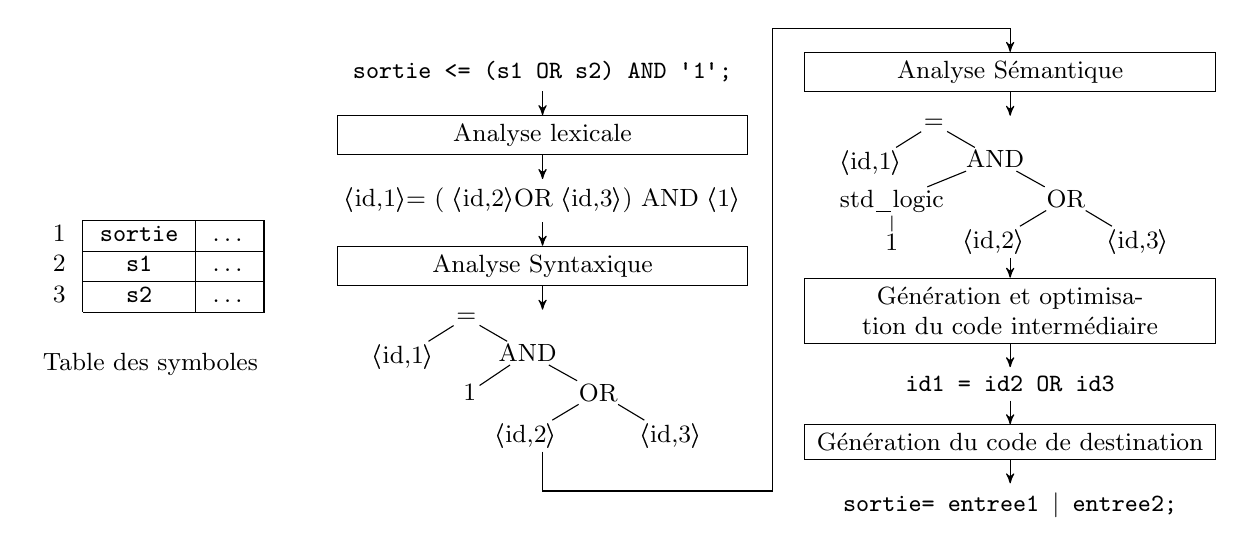
\begin{tikzpicture}[node font=\small, node distance = 0.3cm]
	\node[] (start) {\texttt{sortie <= (s1 OR s2) AND \textquotesingle 1\textquotesingle;}};
	\node[draw, text width = 5cm, text centered,below=of start] (lexical) {Analyse lexicale};
	\node[below=of lexical] (lexicalRes) {\textlangle id,1\textrangle  = ( \textlangle id,2\textrangle OR \textlangle id,3\textrangle ) AND \textlangle 1\textrangle };
	\node[draw, text width = 5cm, text centered,below=of lexicalRes] (Syntax) {Analyse Syntaxique};
	
	
	\begin{scope}[node distance=0.2 and 0.2cm, inner sep=1pt]
	\node[below left = 0.3cm and 0.8cm of Syntax.south] (SyntaxRes1) {=};
	\node[below left =of SyntaxRes1] (SyntaxRes11) {\textlangle id,1\textrangle};
	\node[below right =of SyntaxRes1] (SyntaxRes2) {AND};
	\node[below right =of SyntaxRes2] (SyntaxRes3) {OR};
	\node[below left =of SyntaxRes3] (SyntaxRes31) {\textlangle id,2\textrangle};
	\node[below right =of SyntaxRes3] (SyntaxRes32) {\textlangle id,3\textrangle};
	
	\node[below left = of SyntaxRes2] (SyntaxRes4) {1};
	
	
	\path[draw] (SyntaxRes1) -- (SyntaxRes2)
	(SyntaxRes1) -- (SyntaxRes11)
	(SyntaxRes2) -- (SyntaxRes3)
	(SyntaxRes2) -- (SyntaxRes4)
	(SyntaxRes3) -- (SyntaxRes31)
	(SyntaxRes3) -- (SyntaxRes32)
	;
	\end{scope}
	
	\node[draw, text width = 5cm, text centered,right = 0.8cm of start] (Semantic) {Analyse S\'emantique};
	%  \node[draw, text width = 5cm, text centered,anchor=north] (Semantic) at ($(Syntax.south |- SyntaxRes32.south) - (0,0.3cm)$) {Analyse S\'emantique};
	
	\begin{scope}[node distance=0.2 and 0.2cm, inner sep = 1pt]
	\node[below left =  0.3cm and 0.8cm of Semantic.south] (SemanticRes1) {=};
	\node[below left =of SemanticRes1] (SemanticRes11) {\textlangle id,1\textrangle};
	\node[below right =of SemanticRes1] (SemanticRes2) {AND};
	\node[below right =of SemanticRes2] (SemanticRes3) {OR};
	\node[below left =of SemanticRes3] (SemanticRes31) {\textlangle id,2\textrangle};
	\node[below right =of SemanticRes3] (SemanticRes32) {\textlangle id,3\textrangle};
	
	\node[below left = of SemanticRes2] (SemanticRes4) {std\_logic};
	\node[below = of SemanticRes4] (SemanticRes5) {1};
	
	
	\path[draw] (SemanticRes1) -- (SemanticRes2)
	(SemanticRes1) -- (SemanticRes11)
	(SemanticRes2) -- (SemanticRes3)
	(SemanticRes2) -- (SemanticRes4)
	(SemanticRes4) -- (SemanticRes5)
	(SemanticRes3) -- (SemanticRes31)
	(SemanticRes3) -- (SemanticRes32)
	;
	\end{scope}
	\node[draw,text width = 5cm, text centered, anchor=north] (codeIntGen) at ($(Semantic.south |- SemanticRes5.south) - (0,0.3cm)$) {G\'en\'eration et optimisation du code interm\'ediaire};
	\node[below=of codeIntGen] (codeIntGenRes) {\texttt{id1 = id2 OR id3}};
	\node[draw,text width = 5cm, text centered, below=of codeIntGenRes] (codeDestGen) {G\'en\'eration du code de destination};
	\node[below=of codeDestGen] (codeDestGenRes) {\texttt{sortie= entree1 \textbar ~entree2;}};
	
	
	\path[->,>=stealth'] (start) edge (lexical)
	(lexical) edge (lexicalRes)
	(lexicalRes) edge (Syntax)
	(Syntax) edge (Syntax.south |- SyntaxRes1.north)
	(Semantic) edge (Semantic.south |- SemanticRes1.north)
	(codeIntGen |- SemanticRes31.south) edge (codeIntGen)
	(codeIntGen) edge (codeIntGenRes)
	(codeIntGenRes) edge (codeDestGen)
	(codeDestGen) edge (codeDestGenRes) 
	;
	\path[->,>=stealth', draw]    (Syntax.south |- SyntaxRes31.south) |- 
	($(start.east |- SyntaxRes31.south) + (0.4,-0.5cm)$) |-
	($(start.east |- Semantic.north) + (0.4,0.3cm) $) -| 
	(Semantic.north)
	;
	\node[left=0.8cm of Syntax] (symbolTable) {
		\begin{tabular}{c|c|c|}
		\cline{2-3}
		1 & \texttt{sortie} & \ldots \\
		\cline{2-3}
		2 & \texttt{s1} & \ldots \\
		\cline{2-3}
		3 & \texttt{s2} & \ldots \\
		\cline{2-3}
		\end{tabular}
	};
	\node[below=of symbolTable] {Table des symboles};
	
	\end{tikzpicture}
  \caption{exemple}
\end{figure}

\todo[inline]{Mettre des trucs utiles}
\fi

\section{Conclusion}
On a bien travaillé

\end{document}          
